\chapter{HmPPCAs results on Splatter data-sets}\label{AP:results}
\section{Simple Splatter data-sets}\label{sec:simple}

\begin{figure}
    \centering
    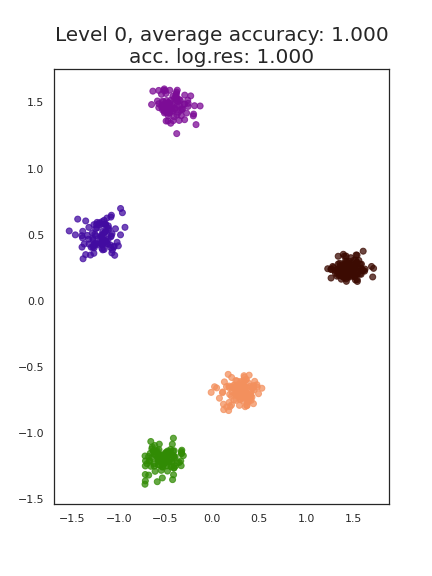
\includegraphics[width=.4\linewidth]{figs/simple_5_nuts.png}
    \caption[HmPPPCAs model performed on the simple Splatter data-set with 5 genes using NUTS]{\small \textbf{HmPPPCAs model performed on the simple Splatter data-set with 5 genes using NUTS.} The maximum accuracy of $1.0$ was found on the top-level. The clusters found within the top-level PPCA have been numbered. The colours indicate different cell types.}
    \label{fig:simple_5_nuts}
\end{figure}

\begin{figure}
    \centering
    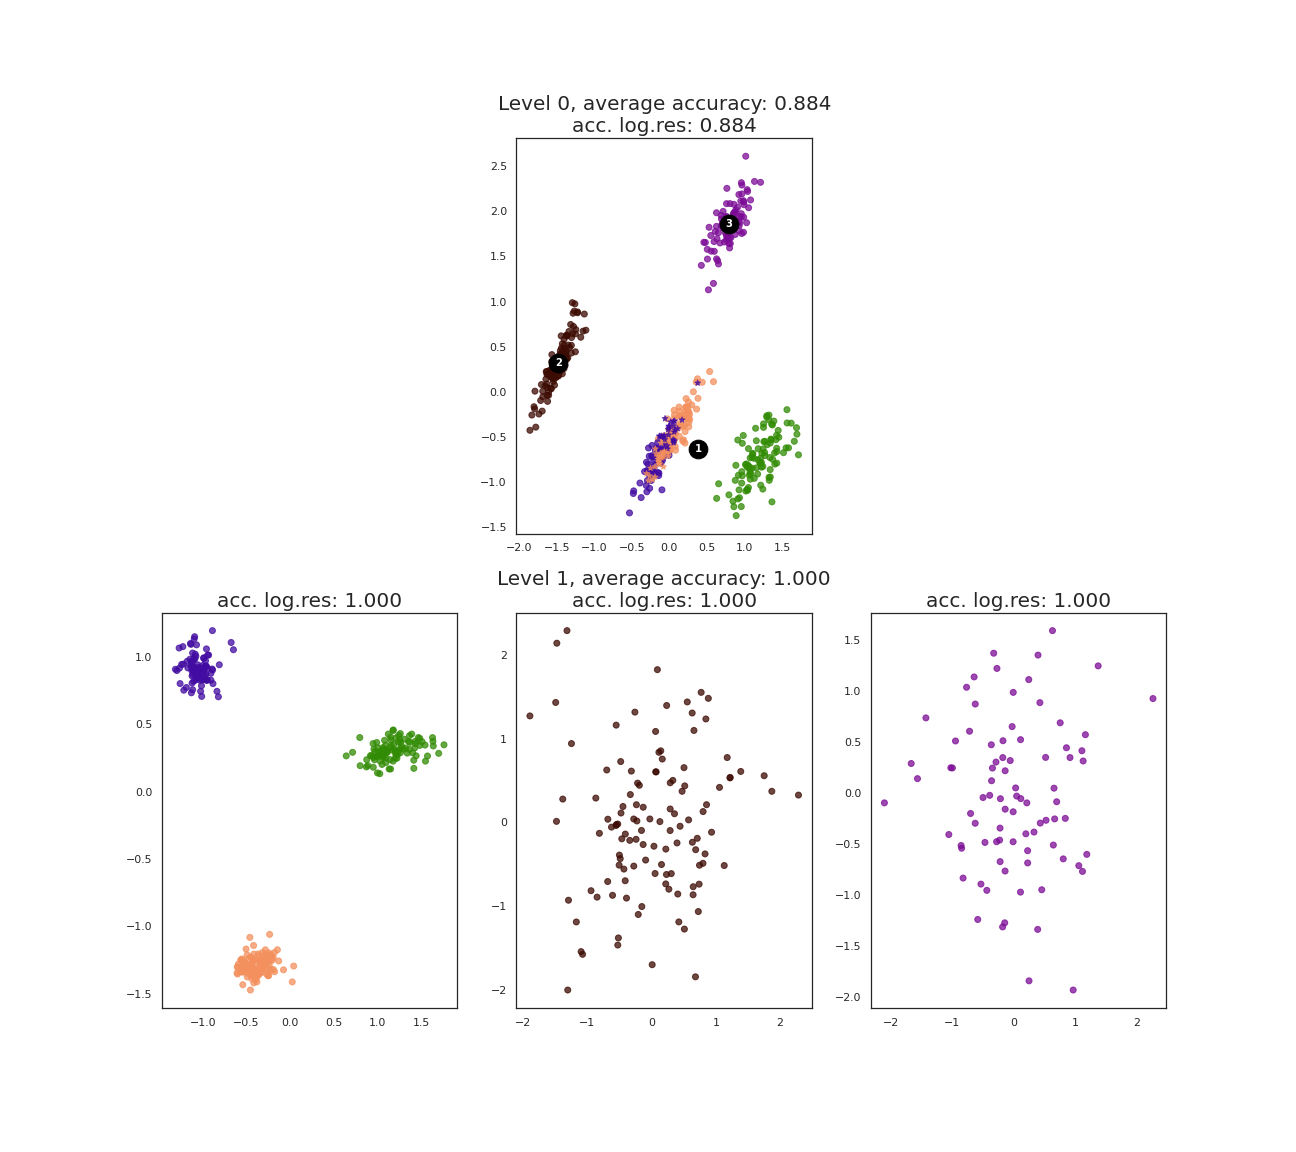
\includegraphics[width=\linewidth]{figs/simple_25_nuts.png}
    \caption[HmPPPCAs model performed on the simple Splatter data-set with 25 genes using NUTS]{\small \textbf{HmPPPCAs model performed on the simple Splatter data-set with 25 genes using NUTS.} \small The maximum accuracy of $1.0$ was found at level $1$. The top-level PPCA achieved an accuracy of $0.884$. The clusters found within the top-level PPCA have been numbered. The colours indicate different cell types. Data-points that were predicted correctly by the logistic regression are plotted with dots, incorrect predictions are plotted with stars.}
    \label{fig:simple_25_nuts}
\end{figure}

\begin{figure}
    \centering
    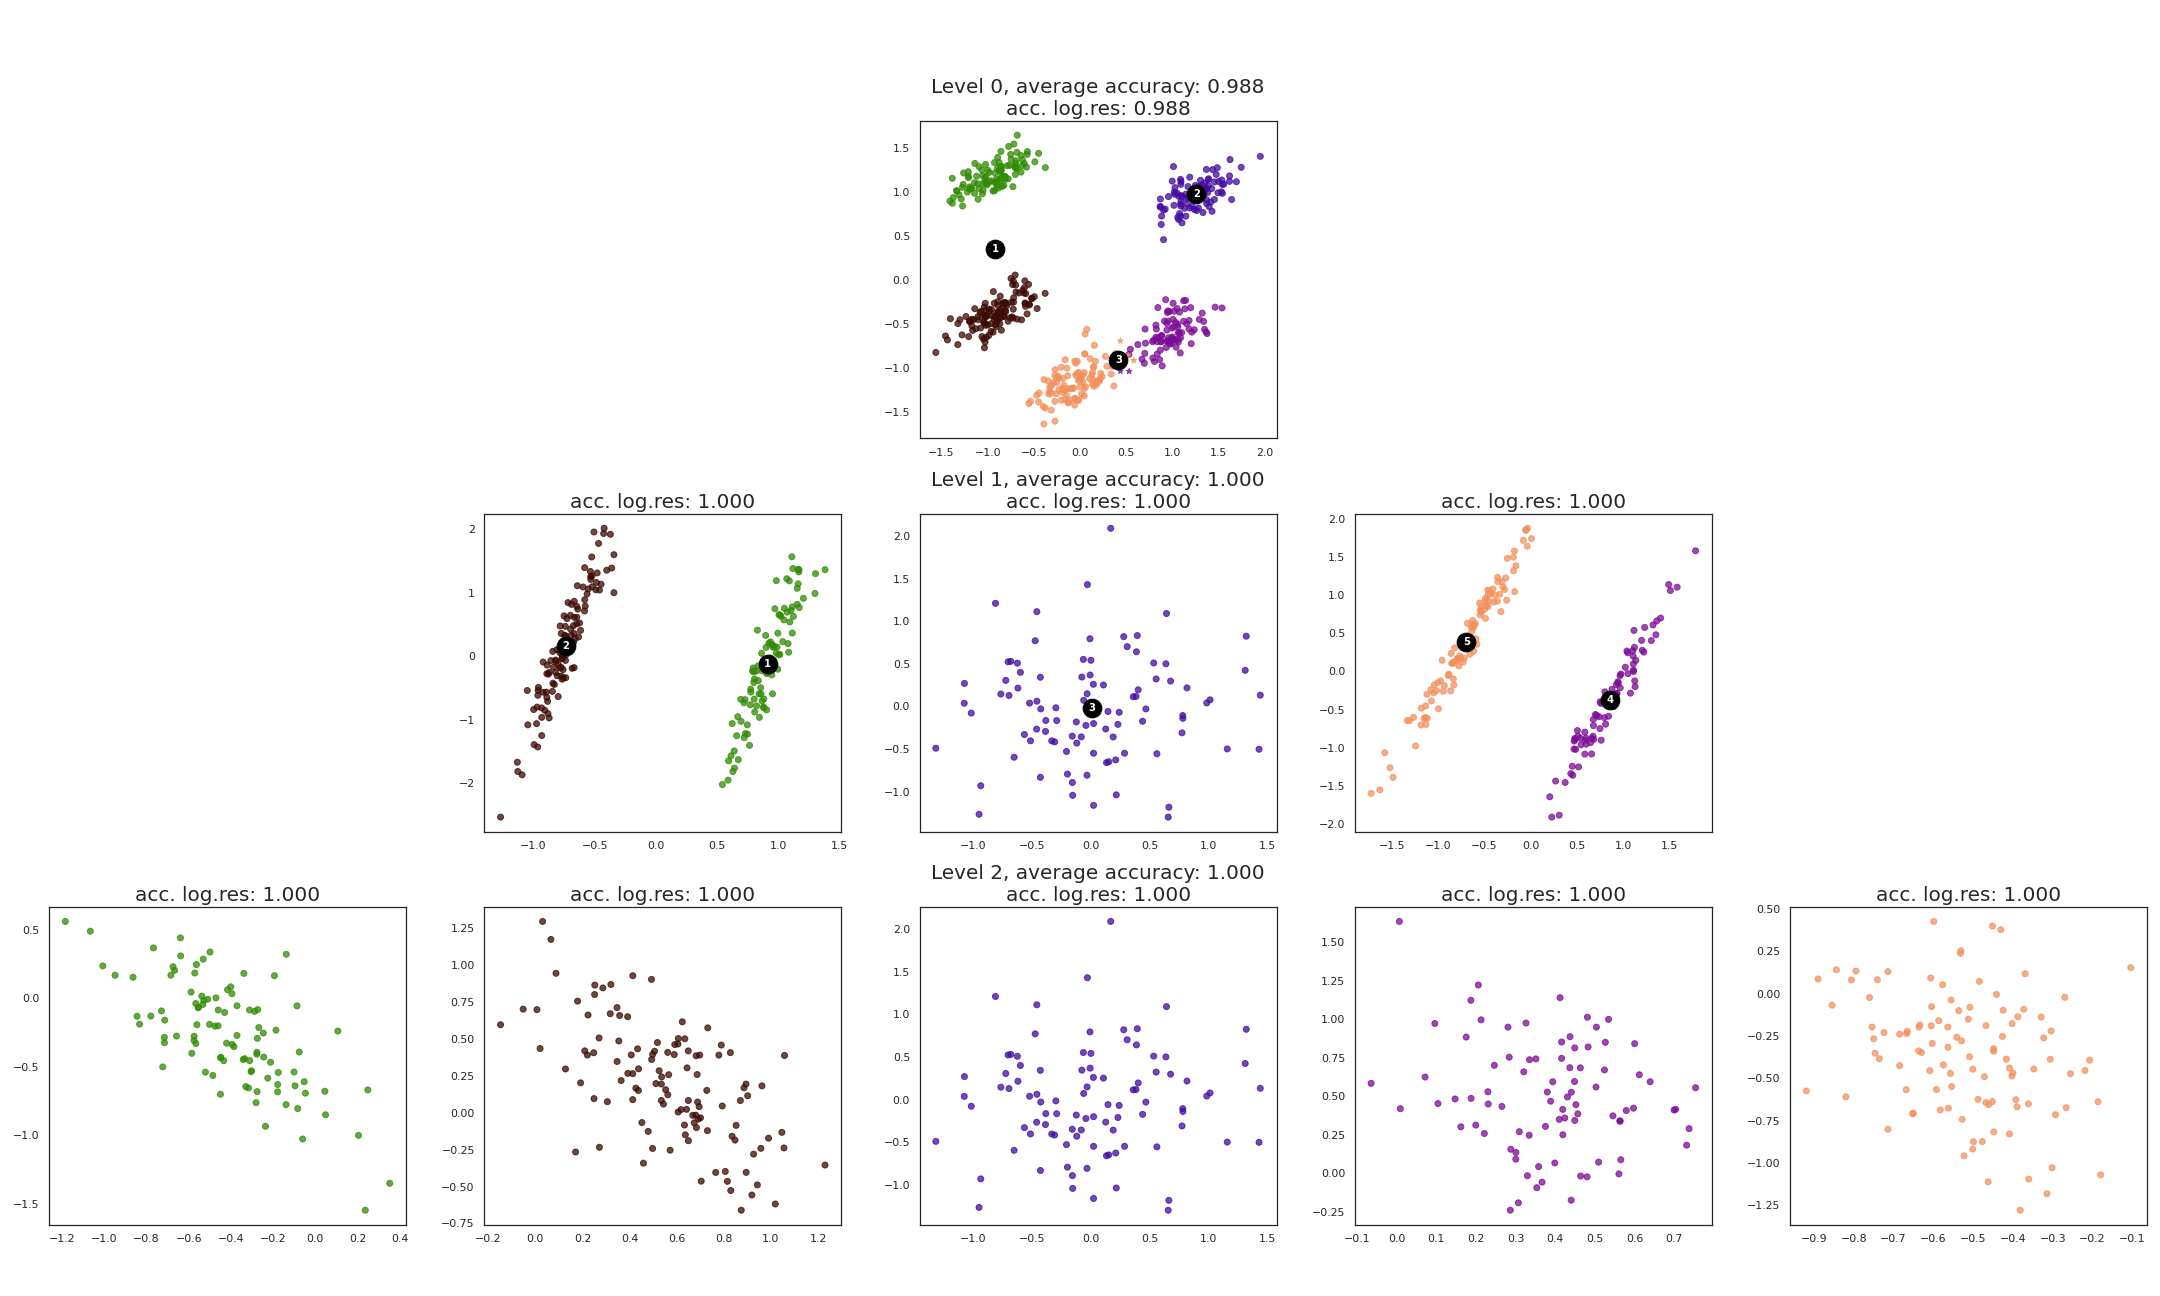
\includegraphics[width=\linewidth]{figs/simple_50_nuts.png}
    \caption[HmPPPCAs model performed on the simple Splatter data-set with 50 genes using NUTS]{\small \textbf{HmPPPCAs model performed on the simple Splatter data-set with 50 genes using NUTS.} \small The maximum accuracy of $1.0$ was found at level $1$. The top-level PPCA achieved an accuracy of $0.988$. The clusters found within the top-level PPCA have been numbered. The colours indicate different cell types. Data-points that were predicted correctly by the logistic regression are plotted with dots, incorrect predictions are plotted with stars.}
    \label{fig:simple_50_nuts}
\end{figure}

\begin{figure}
    \centering
    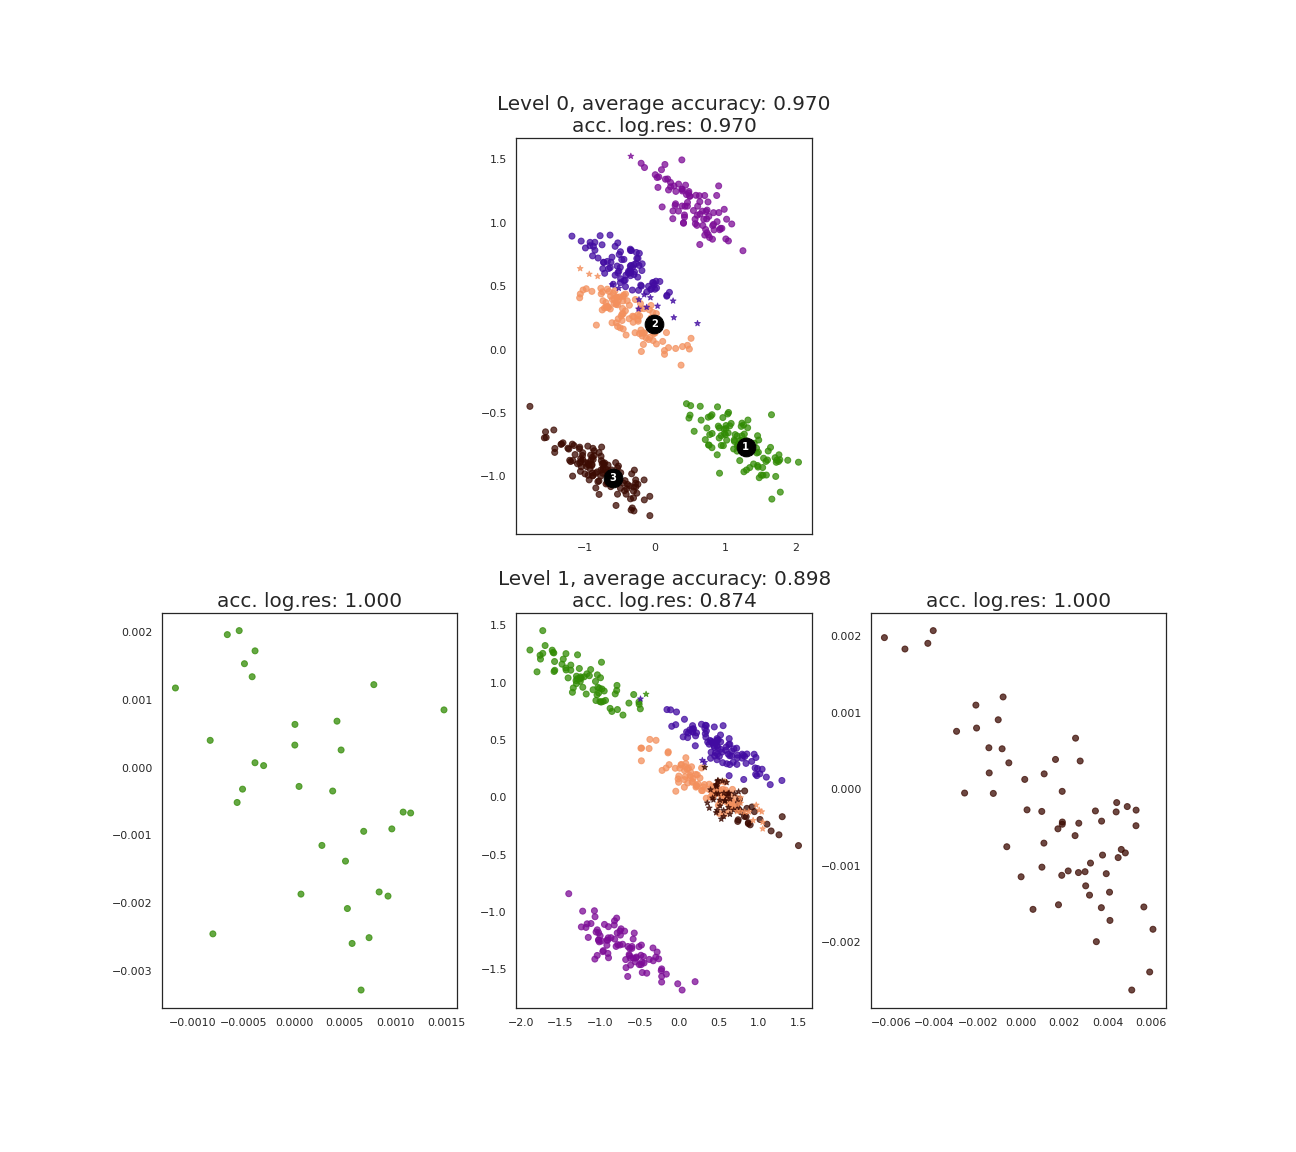
\includegraphics[width=\linewidth]{figs/simple_150_nuts.png}
    \caption[HmPPPCAs model performed on the simple Splatter data-set with 150 genes using NUTS]{\small \textbf{HmPPPCAs model performed on the simple Splatter data-set with 150 genes using NUTS.} \small The maximum accuracy of $0.970$ was found on the top-level. The clusters found within the top-level PPCA have been numbered. The colours indicate different cell types. Data-points that were predicted correctly by the logistic regression are plotted with dots, incorrect predictions are plotted with stars.}
    \label{fig:simple_150_nuts}
\end{figure}

\begin{figure}
    \centering
    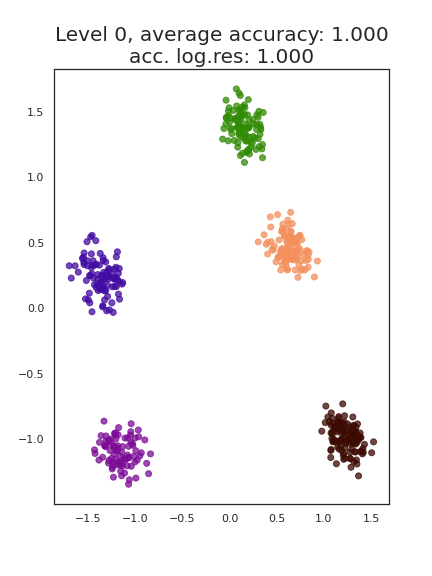
\includegraphics[width=.6\linewidth]{figs/simple_5_vb.png}
    \caption[HmPPPCAs model performed on the simple Splatter data-set with 5 genes using VB]{\small \textbf{HmPPPCAs model performed on the simple Splatter data-set with 5 genes using VB.} \small The maximum accuracy of $1.0$ was found on the top-level. The clusters found within the top-level PPCA have been numbered. The colours indicate different cell types.}
    \label{fig:simple_5_vb}
\end{figure}

\begin{figure}
    \centering
    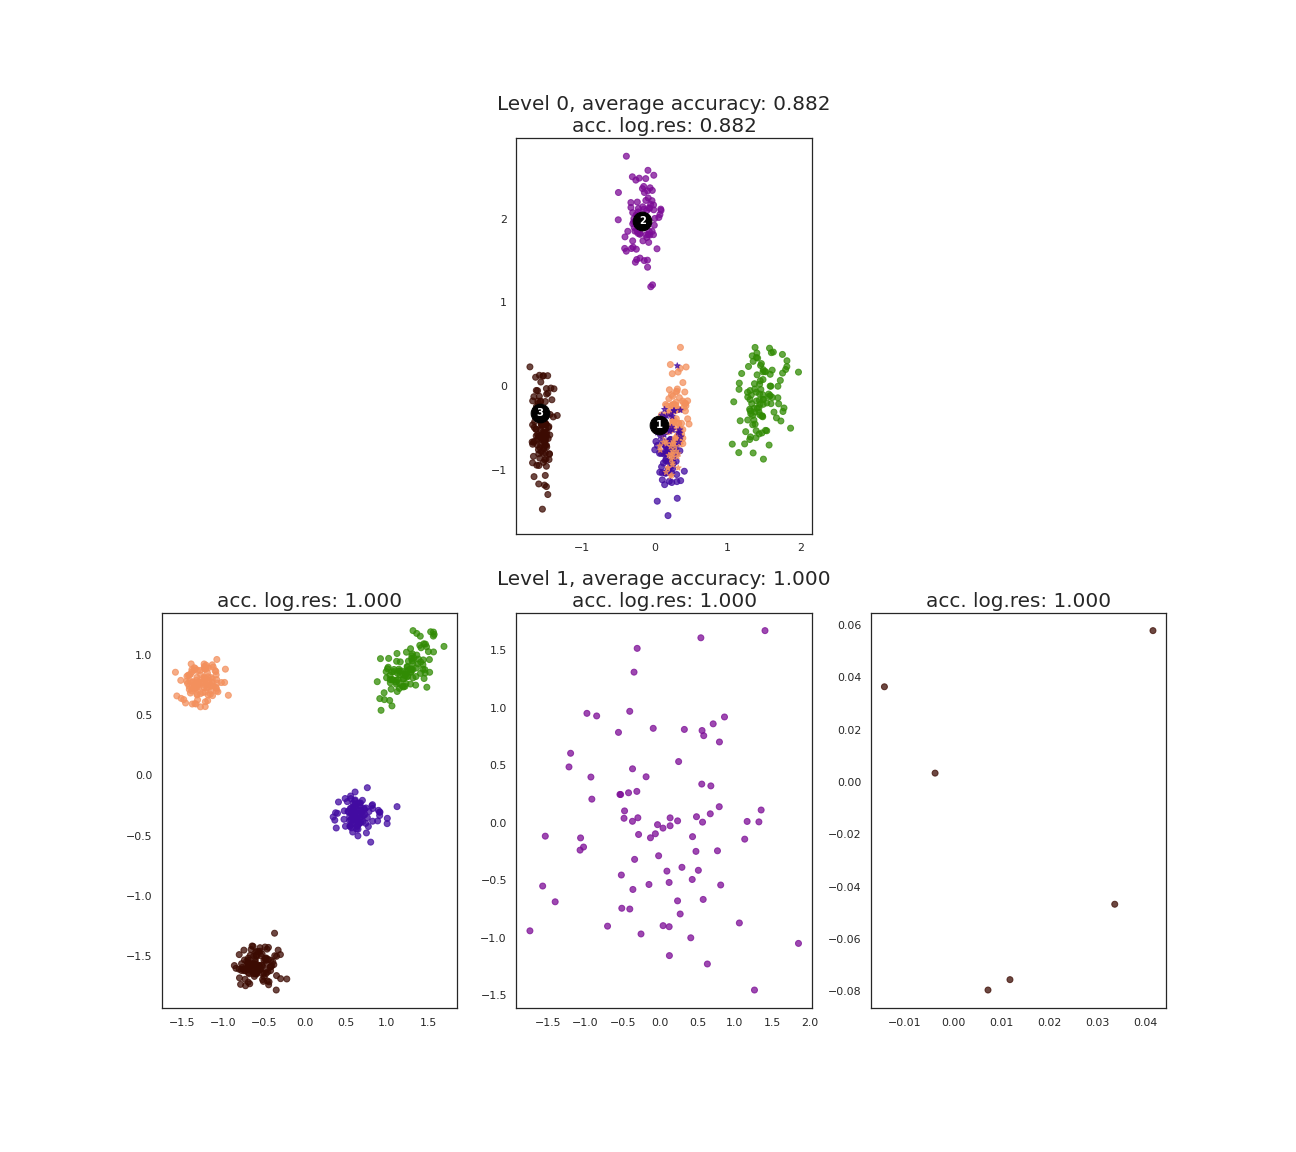
\includegraphics[width=\linewidth]{figs/simple_25_vb.png}
    \caption[HmPPPCAs model performed on the simple Splatter data-set with 25 genes using VB]{\small \textbf{HmPPPCAs model performed on the simple Splatter data-set with 25 genes using VB.} \small The maximum accuracy of $1.0$ was found at level $1$. The top-level PPCA achieved an accuracy of $0.882$. The clusters found within the top-level PPCA have been numbered. The colours indicate different cell types. Data-points that were predicted correctly by the logistic regression are plotted with dots, incorrect predictions are plotted with stars.}
    \label{fig:simple_25_vb}
\end{figure}

\begin{figure}
    \centering
    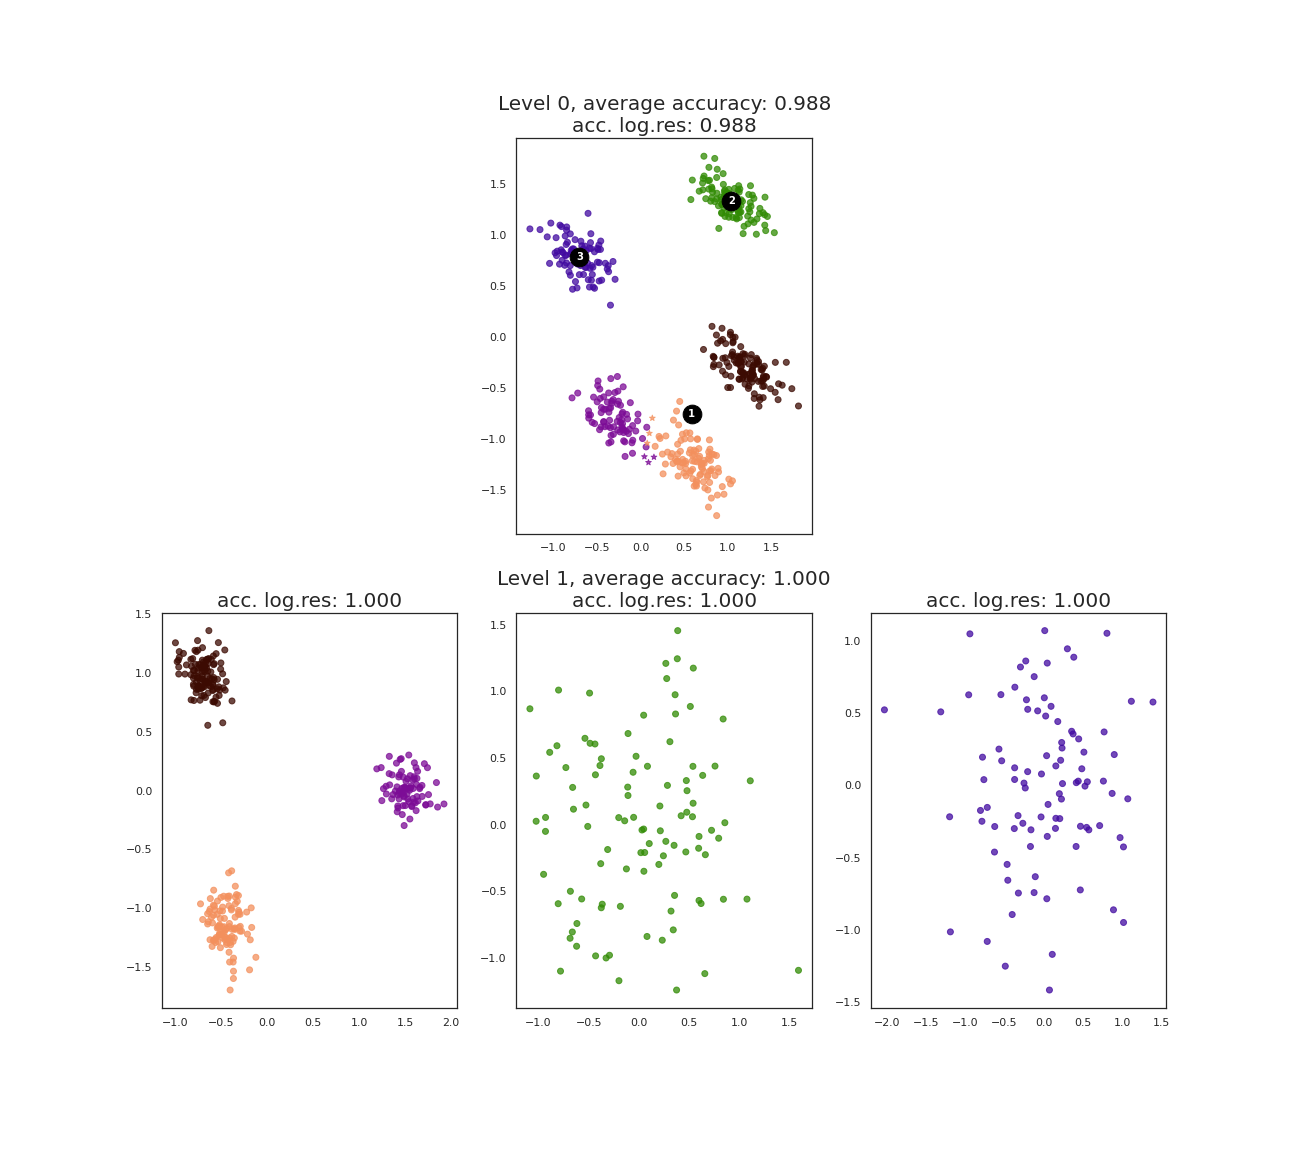
\includegraphics[width=\linewidth]{figs/simple_50_vb.png}
    \caption[HmPPPCAs model performed on the simple Splatter data-set with 50 genes using VB]{\small \textbf{HmPPPCAs model performed on the simple Splatter data-set with 50 genes using VB.} \small The maximum accuracy of $1.0$ was found at level $1$. The top-level PPCA achieved an accuracy of $0.988$. The clusters found within the top-level PPCA have been numbered. The colours indicate different cell types. Data-points that were predicted correctly by the logistic regression are plotted with dots, incorrect predictions are plotted with stars.}
    \label{fig:simple_50_vb}
\end{figure}

\begin{figure}
    \centering
    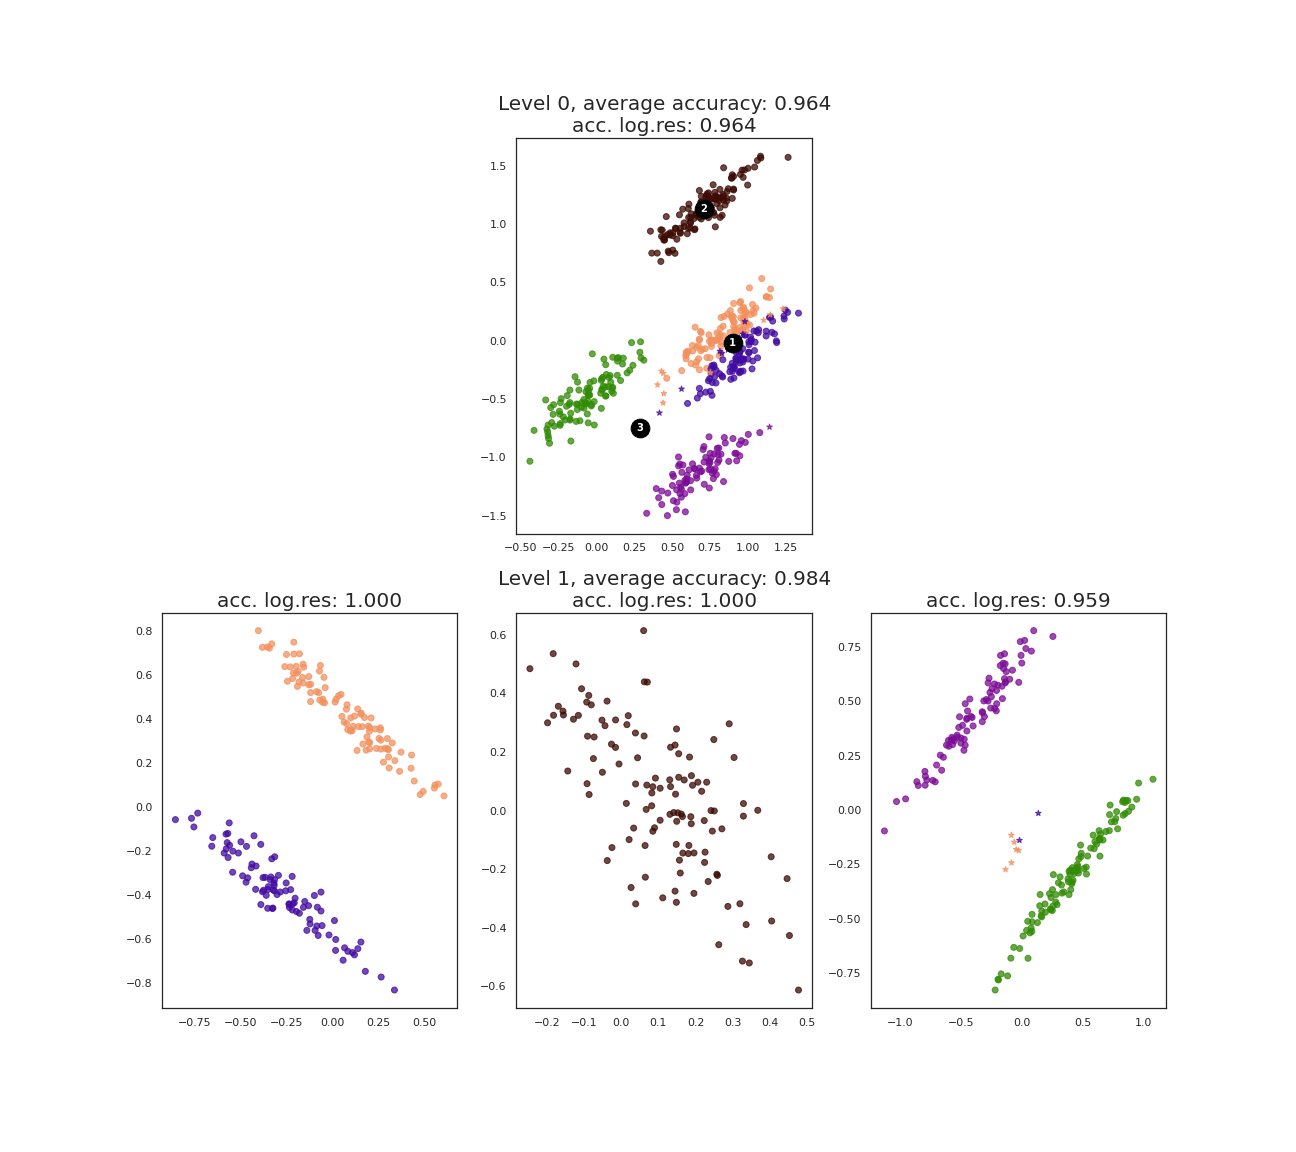
\includegraphics[width=\linewidth]{figs/simple_150_vb.png}
    \caption[HmPPPCAs model performed on the simple Splatter data-set with 150 genes using VB]{\small \textbf{HmPPPCAs model performed on the simple Splatter data-set with 150 genes using VB.} \small The maximum accuracy of $0.984$ was found at level $1$. The top-level PPCA achieved an accuracy of $0.964$. The clusters found within the top-level PPCA have been numbered. The colours indicate different cell types. Data-points that were predicted correctly by the logistic regression are plotted with dots, incorrect predictions are plotted with stars.}
    \label{fig:simple_150_vb}
\end{figure}

\clearpage
% \newpage

\section{Complex Splatter data-sets}\label{sec:complex}

\begin{figure}[h]
    \centering
    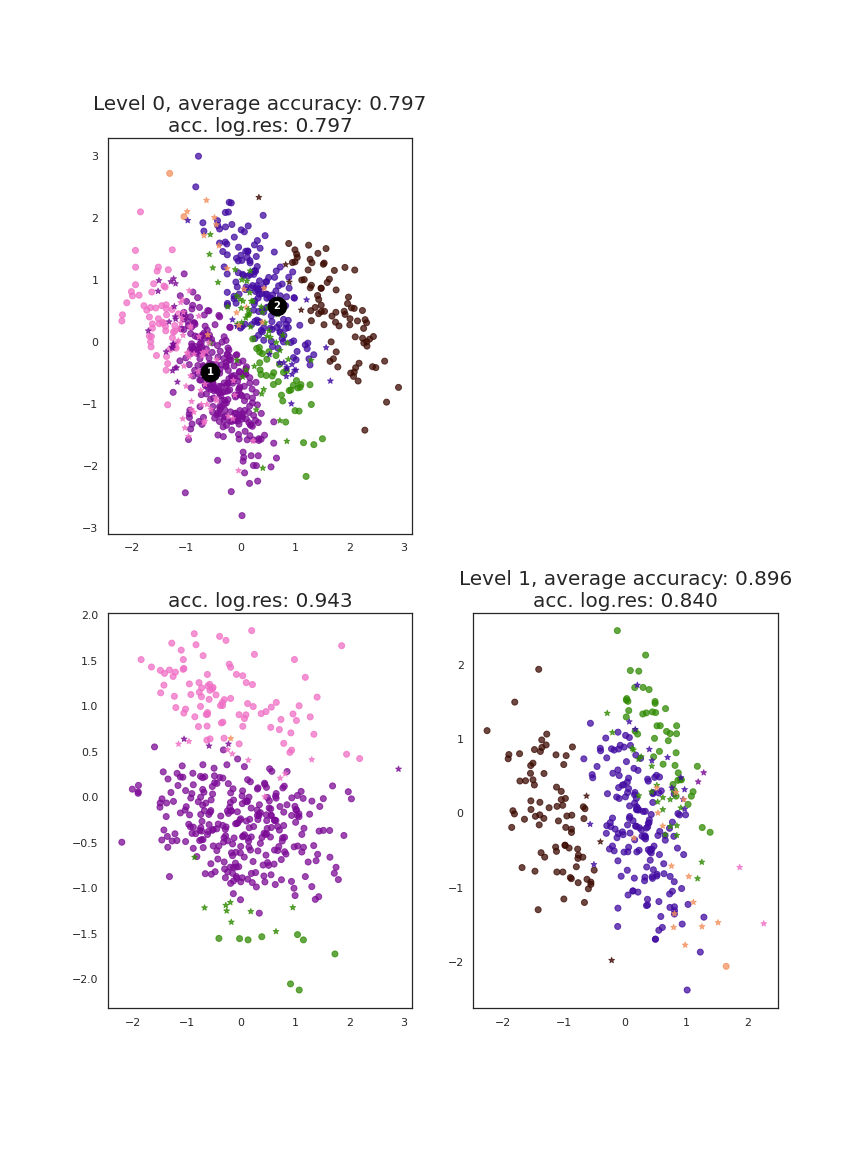
\includegraphics[width=.8\linewidth]{figs/complex_5_nuts.png}
    \caption[HmPPPCAs model performed on the complex Splatter data-set with 5 genes using NUTS]{\small \textbf{HmPPPCAs model performed on the complex Splatter data-set with 5 genes using NUTS.} \small The maximum accuracy of $0.896$ was found at level $1$. The top-level PPCA achieved an accuracy of $0.797$. The clusters found within the top-level PPCA have been numbered. The colours indicate different cell types. Data-points that were predicted correctly by the logistic regression are plotted with dots, incorrect predictions are plotted with stars.}
    \label{fig:complex_5_nuts}
\end{figure}

\begin{figure}
    \centering
    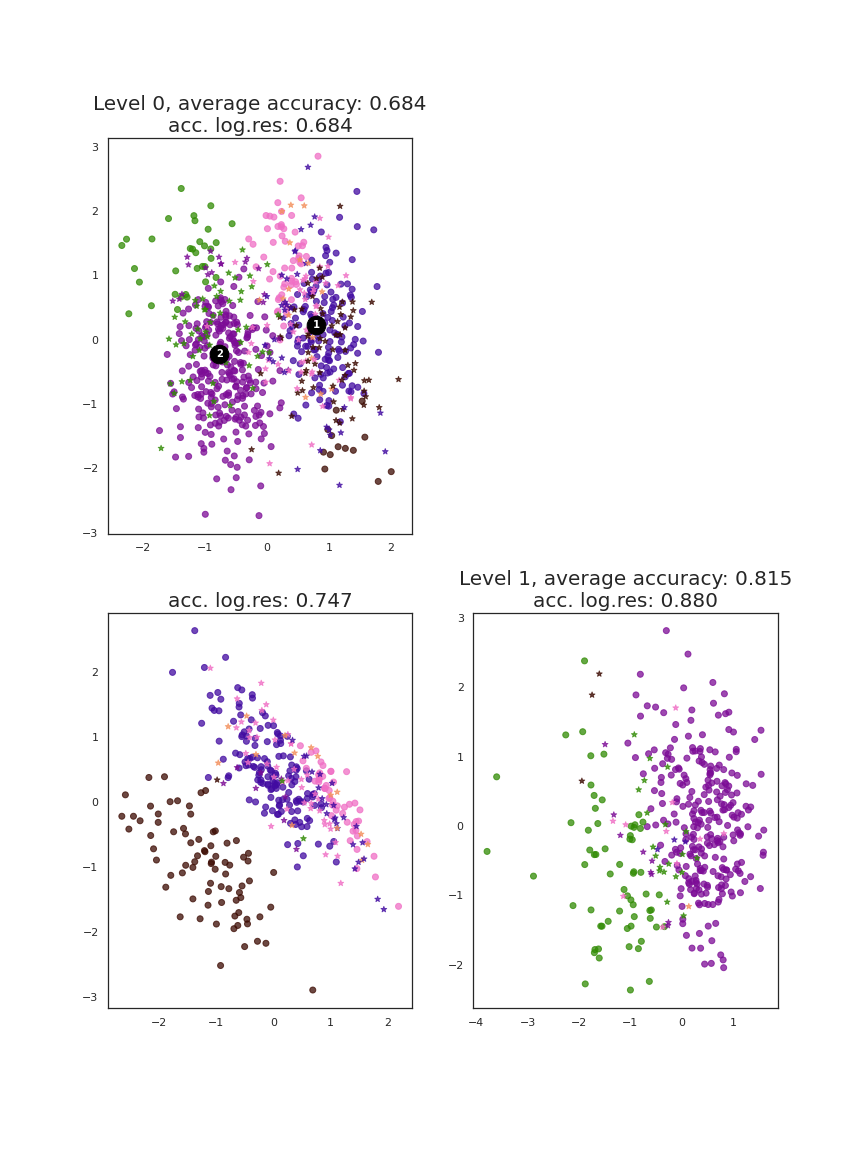
\includegraphics[width=\linewidth]{figs/complex_25_nuts.png}
    \caption[HmPPPCAs model performed on the complex Splatter data-set with 25 genes using NUTS]{\small \textbf{HmPPPCAs model performed on the complex Splatter data-set with 25 genes using NUTS.} \small The maximum accuracy of $0.815$ was found at level $1$. The top-level PPCA achieved an accuracy of $0.684$. The clusters found within the top-level PPCA have been numbered. The colours indicate different cell types. Data-points that were predicted correctly by the logistic regression are plotted with dots, incorrect predictions are plotted with stars.}
    \label{fig:complex_25_nuts}
\end{figure}

\begin{figure}
    \centering
    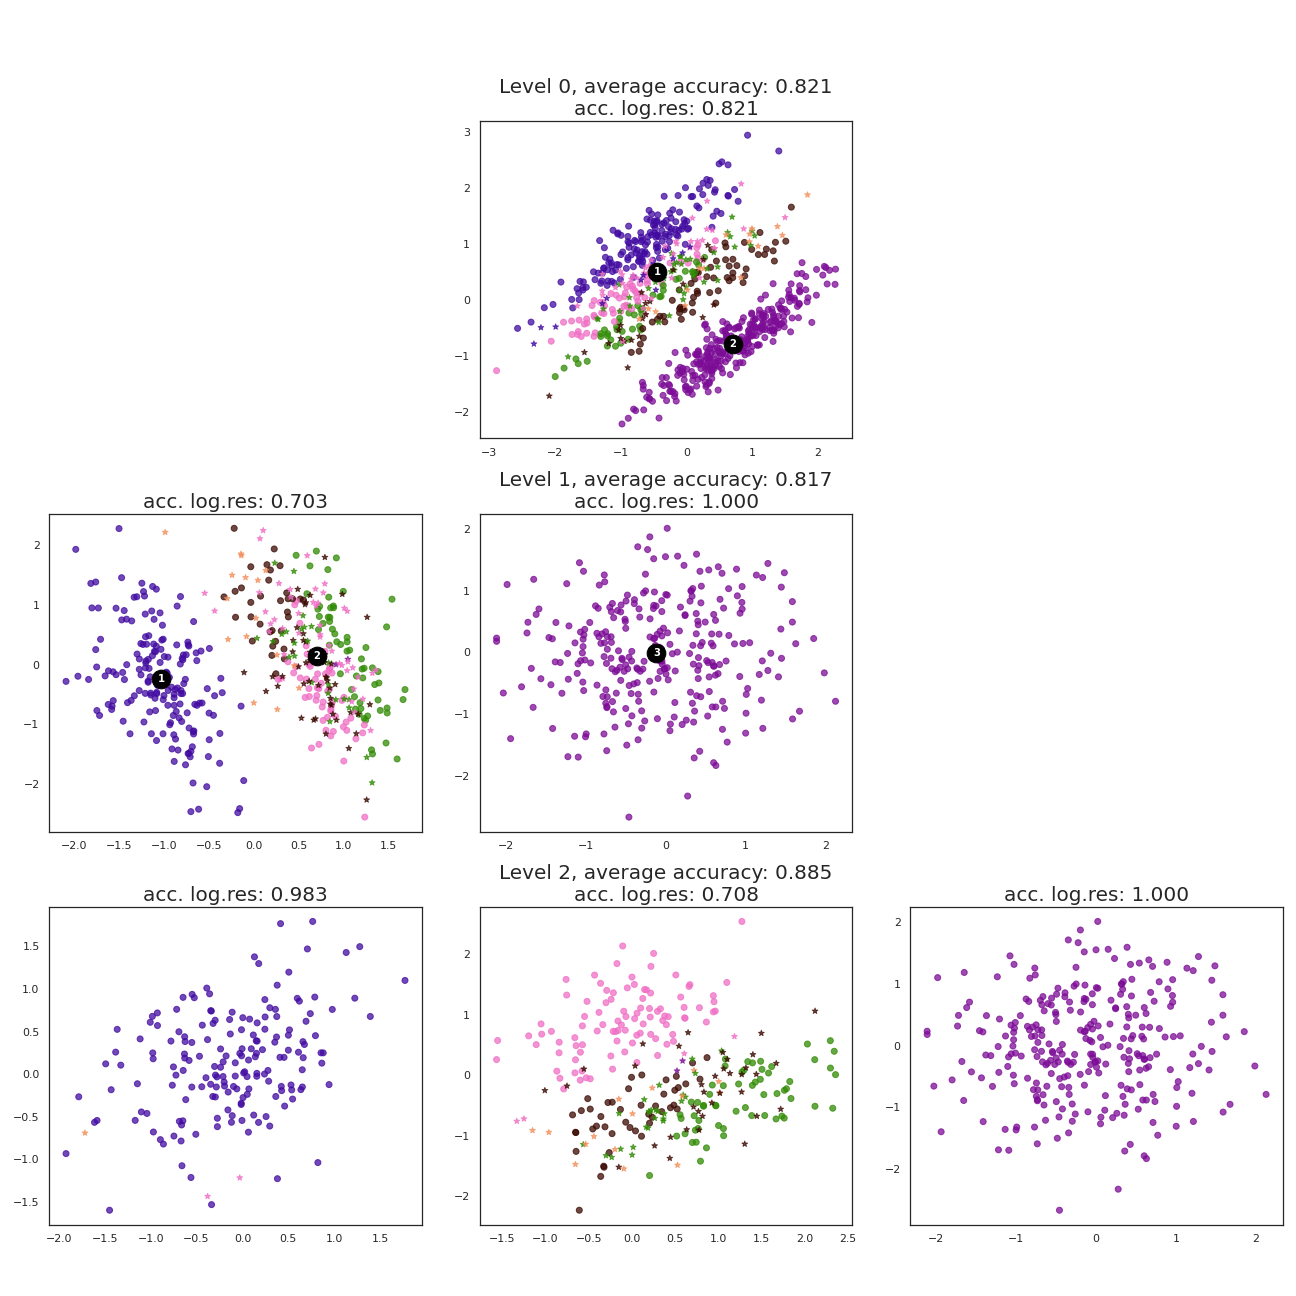
\includegraphics[width=\linewidth]{figs/complex_50_nuts.png}
    \caption[HmPPPCAs model performed on the complex Splatter data-set with 50 genes using NUTS]{\small \textbf{HmPPPCAs model performed on the complex Splatter data-set with 50 genes using NUTS.} \small The maximum accuracy of $0.885$ was found at level $2$. The top-level PPCA achieved an accuracy of $0.821$. The clusters found within each level have been numbered. The colours indicate different cell types. Data-points that were predicted correctly by the logistic regression are plotted with dots, incorrect predictions are plotted with stars.}
    \label{fig:complex_50_nuts}
\end{figure}

\begin{figure}
    \centering
    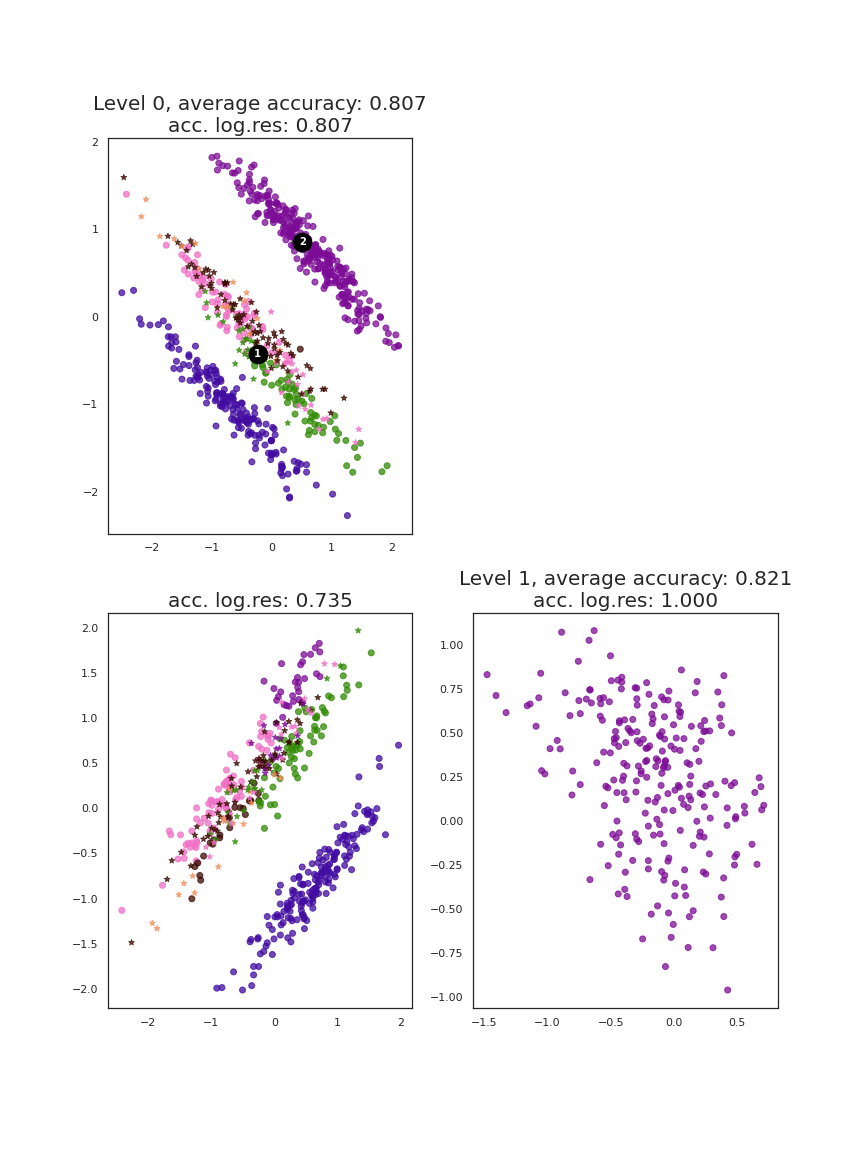
\includegraphics[width=\linewidth]{figs/complex_150_nuts.png}
    \caption[HmPPPCAs model performed on the complex Splatter data-set with 150 genes using NUTS]{\small \textbf{HmPPPCAs model performed on the complex Splatter data-set with 150 genes using NUTS.} \small The maximum accuracy of $0.821$ was found at level $1$. The top-level PPCA achieved an accuracy of $0.807$. The clusters found within the top-level PPCA have been numbered. The colours indicate different cell types. Data-points that were predicted correctly by the logistic regression are plotted with dots, incorrect predictions are plotted with stars.}
    \label{fig:complex_150_nuts}
\end{figure}



\begin{figure}
    \centering
    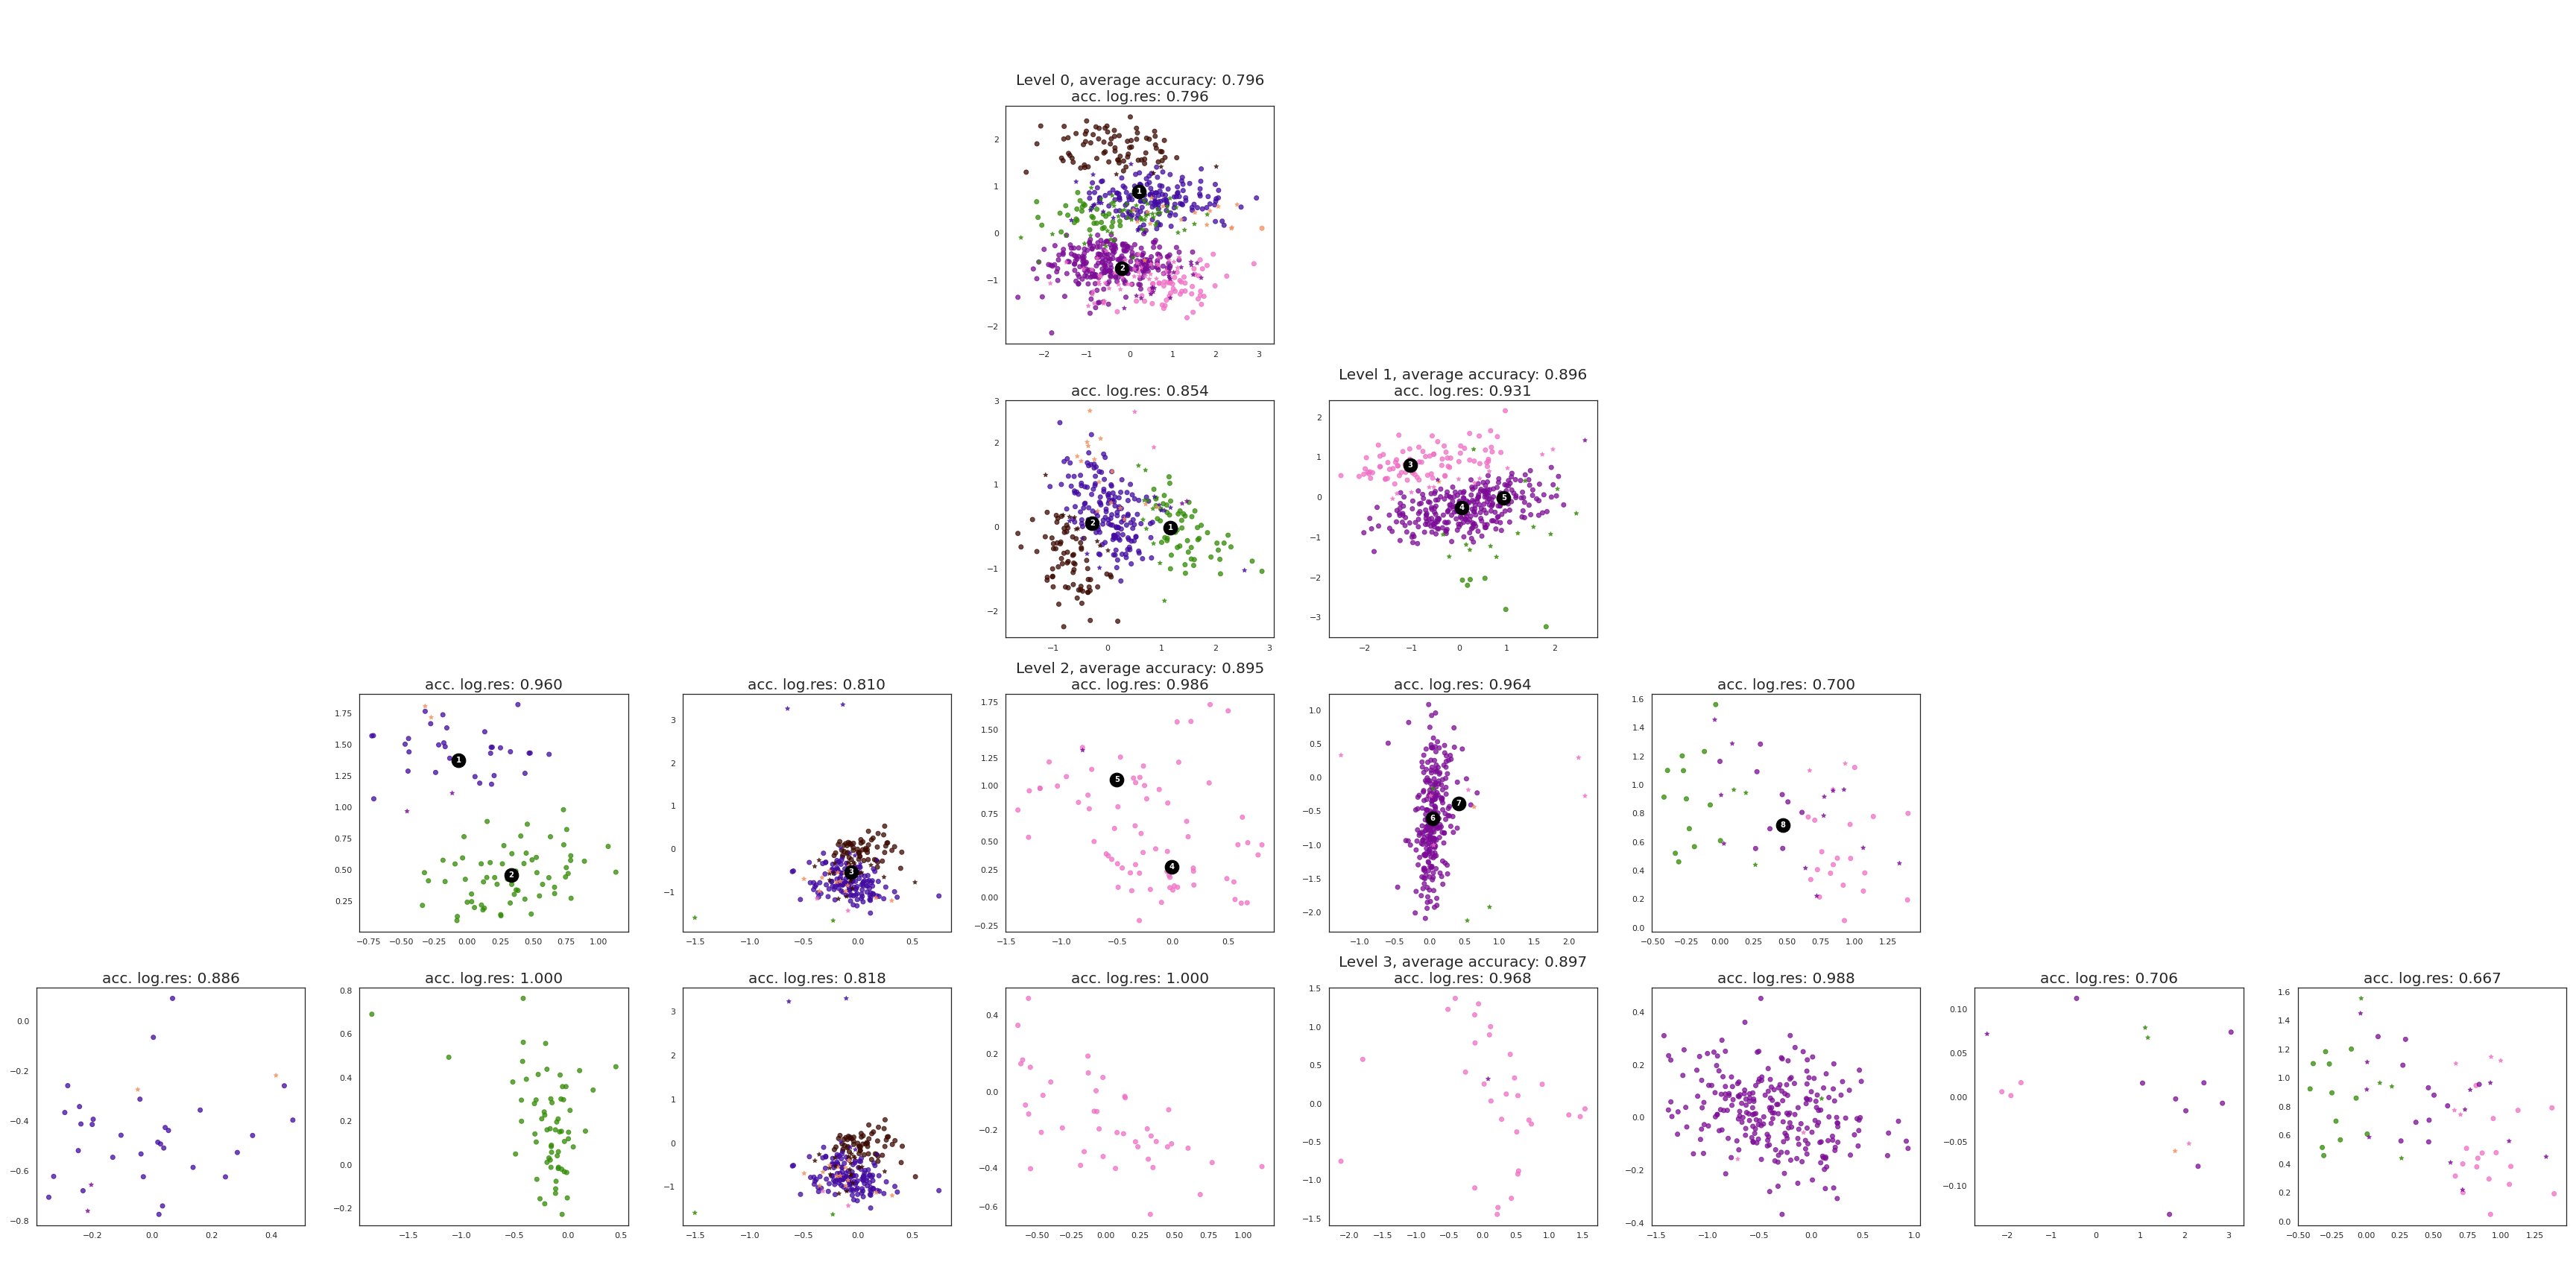
\includegraphics[width=\linewidth]{figs/complex_5_vb.png}
    \caption[HmPPPCAs model performed on the complex Splatter data-set with 5 genes using VB]{\small \textbf{HmPPPCAs model performed on the complex Splatter data-set with 5 genes using VB.} \small The maximum accuracy of $0.897$ was found at level $3$. The top-level PPCA achieved an accuracy of $0.796$. The clusters found within each level have been numbered. The colours indicate different cell types. Data-points that were predicted correctly by the logistic regression are plotted with dots, incorrect predictions are plotted with stars.}
    \label{fig:complex_5_vb}
\end{figure}

\begin{figure}
    \centering
    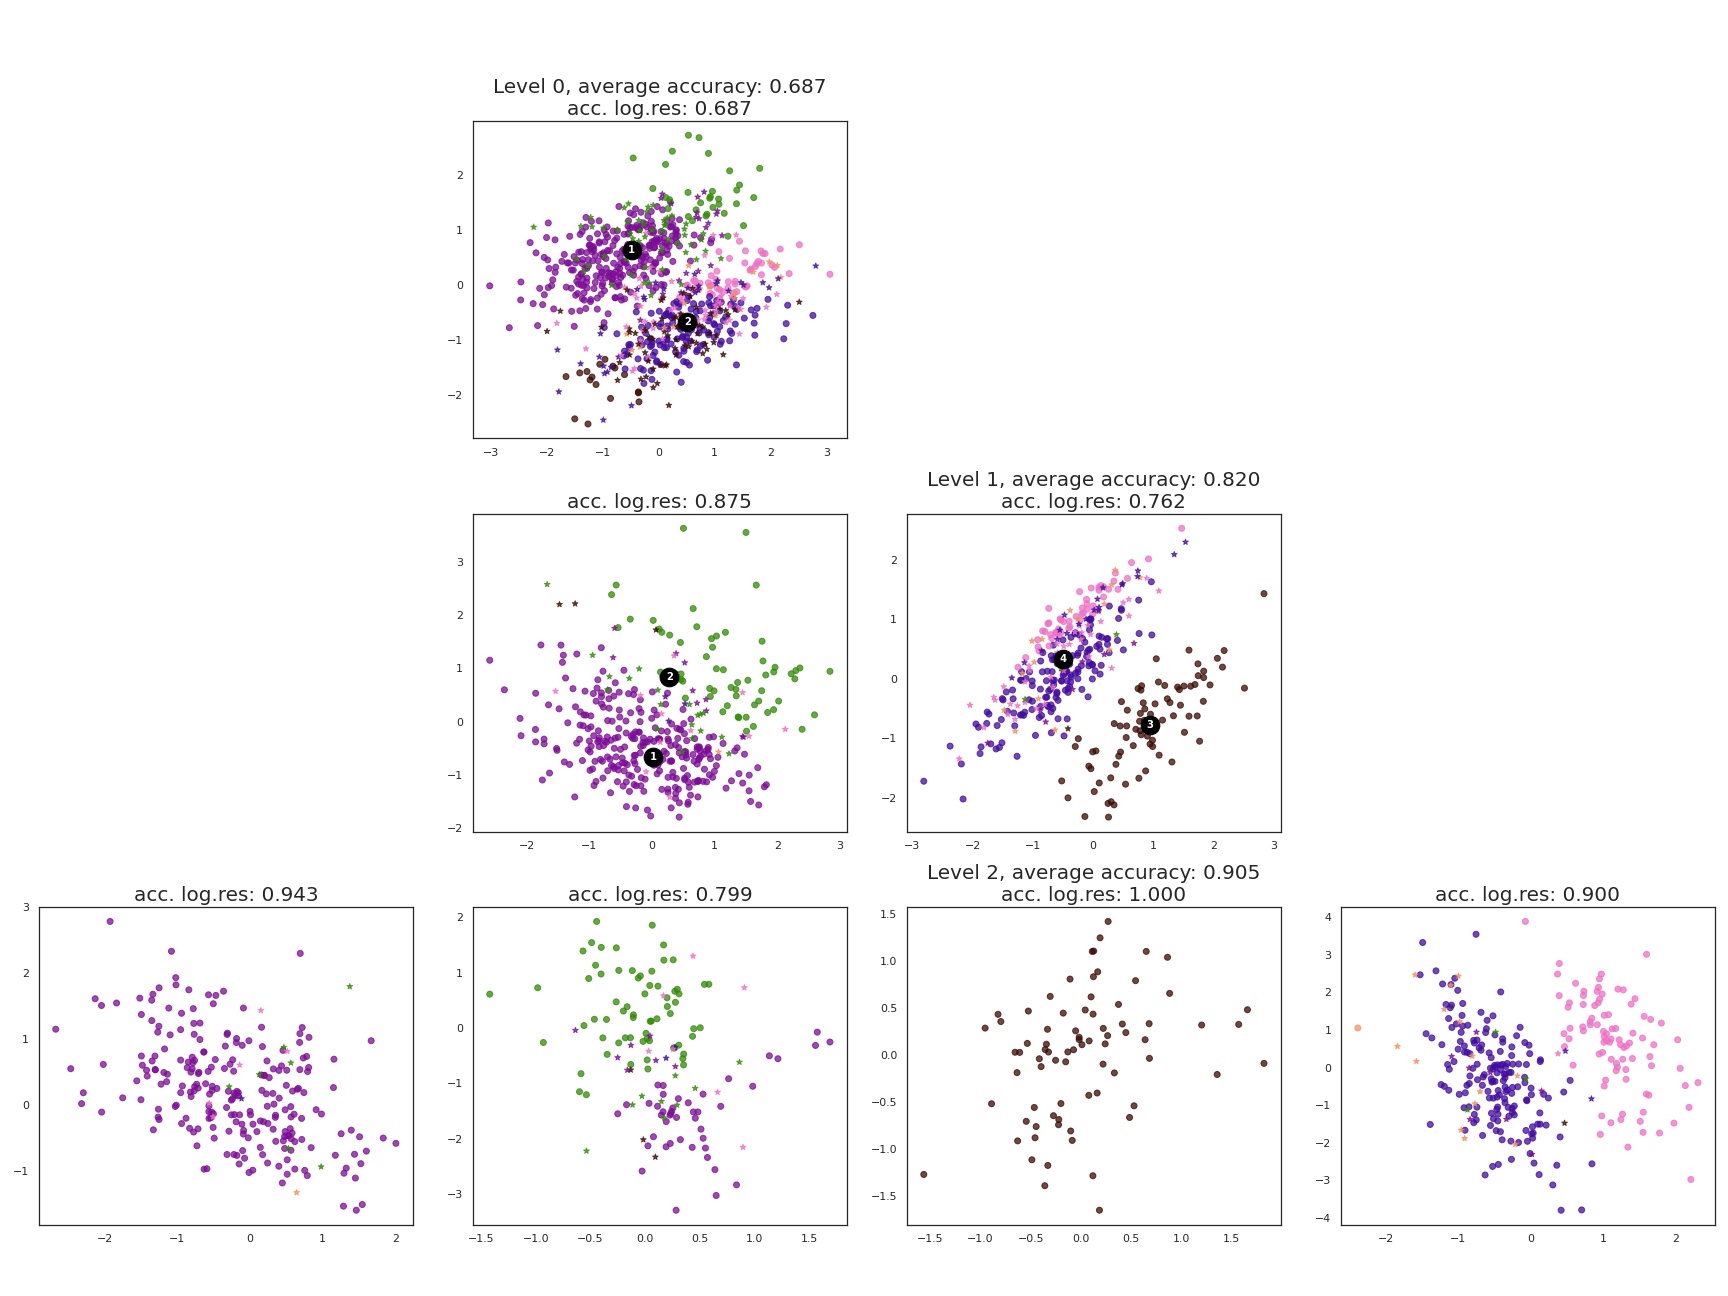
\includegraphics[width=\linewidth]{figs/complex_25_vb.png}
    \caption[HmPPPCAs model performed on the complex Splatter data-set with 25 genes using VB]{\small \textbf{HmPPPCAs model performed on the complex Splatter data-set with 25 genes using VB.} \small The maximum accuracy of $0.905$ was found at level $2$. The top-level PPCA achieved an accuracy of $0.687$. The clusters found within each level have been numbered. The colours indicate different cell types. Data-points that were predicted correctly by the logistic regression are plotted with dots, incorrect predictions are plotted with stars.}
    \label{fig:complex_25_vb}
\end{figure}

\begin{figure}
    \centering
    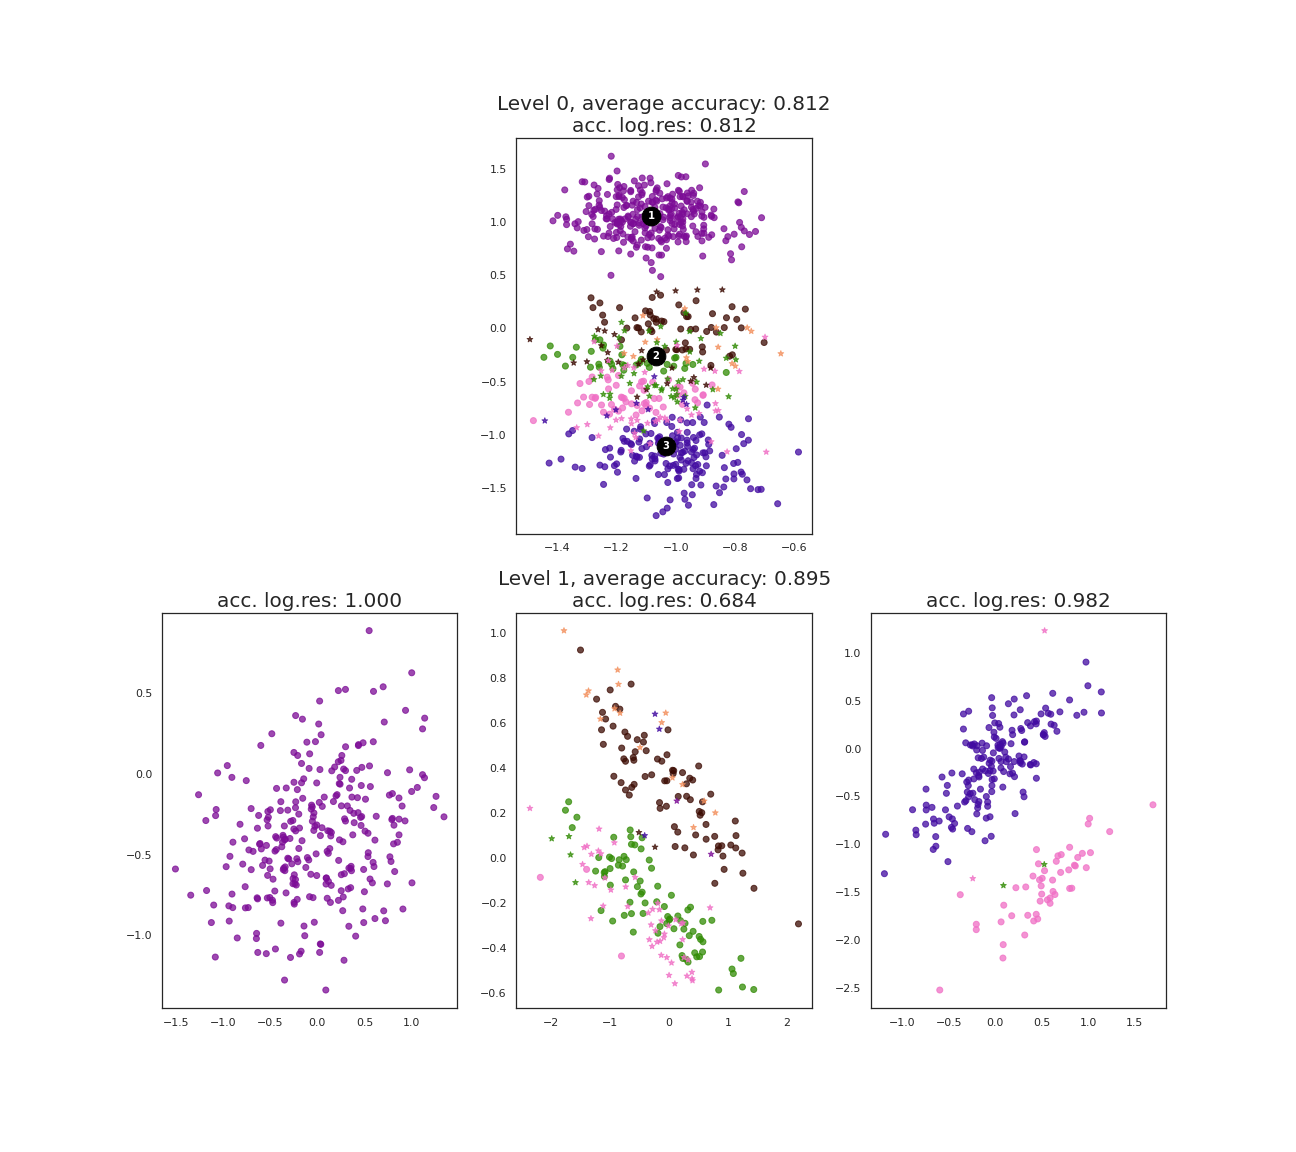
\includegraphics[width=\linewidth]{figs/complex_50_vb.png}
    \caption[HmPPPCAs model performed on the complex Splatter data-set with 50 genes using VB]{\small \textbf{HmPPPCAs model performed on the complex Splatter data-set with 50 genes using VB.} \small The maximum accuracy of $0.895$ was found at level $1$. The top-level PPCA achieved an accuracy of $0.812$. The clusters found within the top-level PPCA have been numbered. The colours indicate different cell types. Data-points that were predicted correctly by the logistic regression are plotted with dots, incorrect predictions are plotted with stars.}
    \label{fig:complex_50_vb}
\end{figure}

\begin{figure}
    \centering
    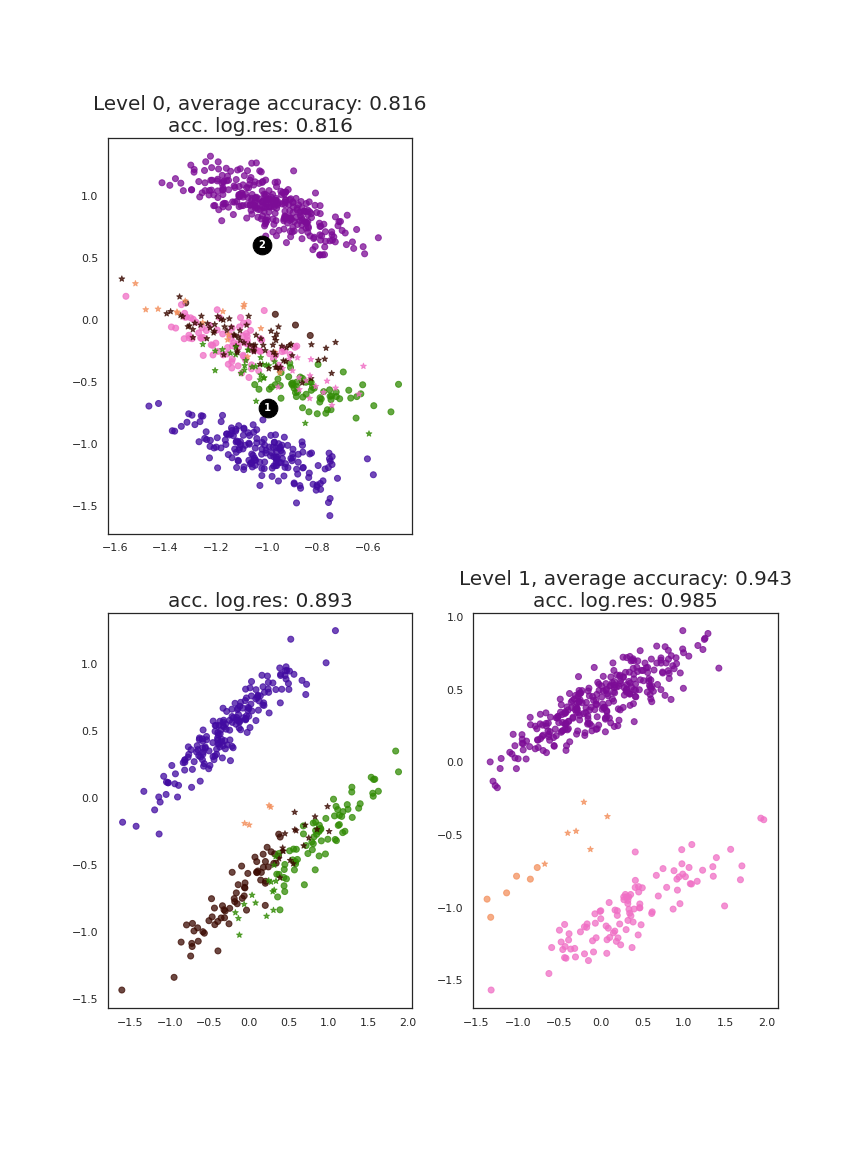
\includegraphics[width=\linewidth]{figs/complex_150_vb.png}
    \caption[HmPPPCAs model performed on the complex Splatter data-set with 150 genes using VB]{\small \textbf{HmPPPCAs model performed on the complex Splatter data-set with 150 genes using VB.} \small The maximum accuracy of $0.943$ was found at level $1$. The top-level PPCA achieved an accuracy of $0.816$. The clusters found within the top-level PPCA have been numbered. The colours indicate different cell types. Data-points that were predicted correctly by the logistic regression are plotted with dots, incorrect predictions are plotted with stars.}
    \label{fig:complex_150_vb}
\end{figure}

\clearpage
% \newpage

\section{UMAP and t-SNE results on the Splatter data-sets}\label{sec:baselineresults}


\begin{figure}[h]
\centering
\begin{subfigure}{.3\textwidth}
  \centering
  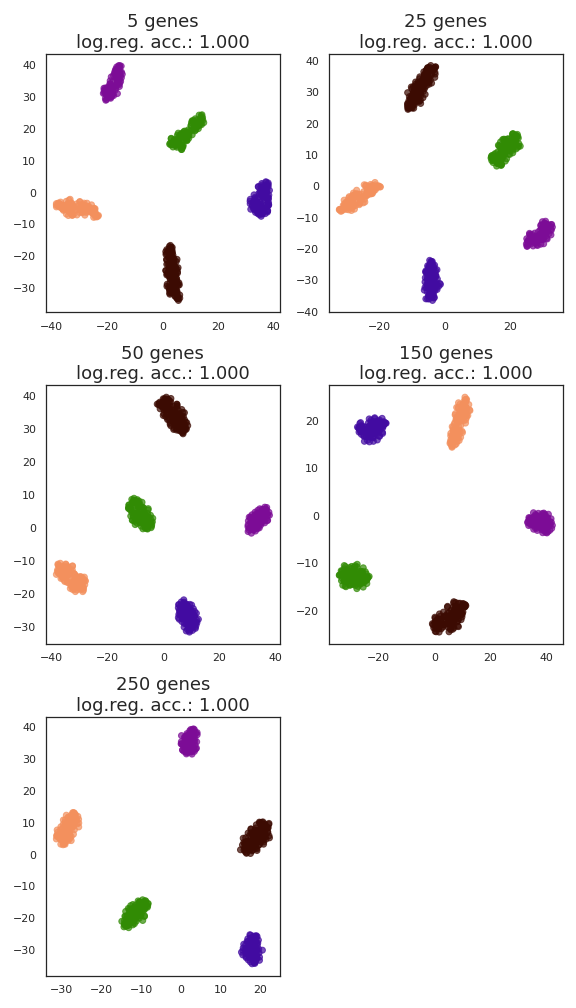
\includegraphics[width=\linewidth]{figs/TSNE_simple.png}
  \caption{\small t-SNE performance on the simple Splatter data-sets}
  \label{fig:tmse_simple}
\end{subfigure}\hspace{30px}%
\begin{subfigure}{.3\textwidth}
  \centering
  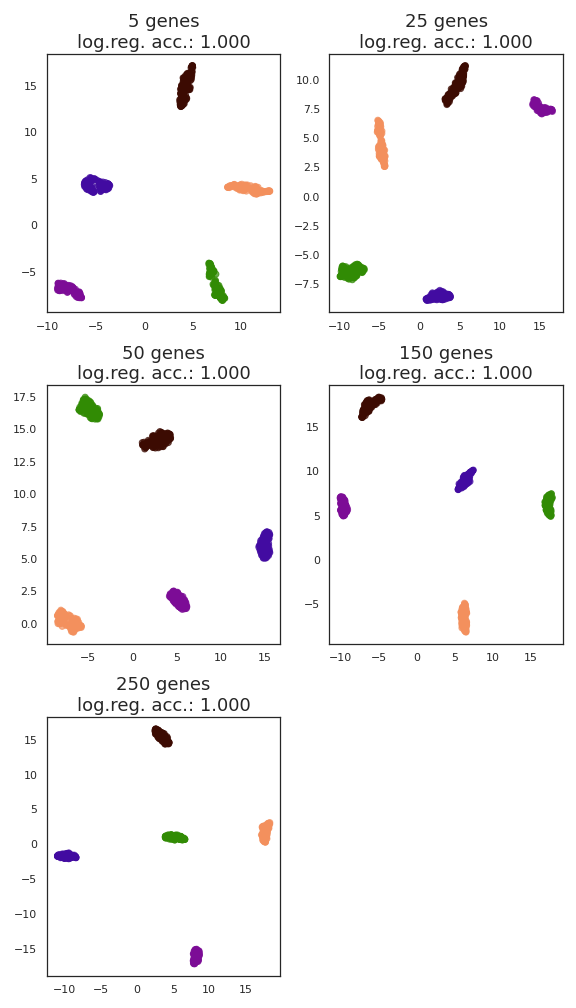
\includegraphics[width=\linewidth]{figs/UMAP_simple.png}
  \caption{\small UMAP performance on the simple Splatter data-sets}
  \label{fig:umap_simple}
\end{subfigure}
% \small
% \caption[t-SNE (left) and UMAP (right) performance on the simple Splatter data-sets.]{\small \textbf{t-SNE (left) and UMAP (right) performance on the simple Splatter data-sets.} \small
% In both figures, the plot with colours based on the original labels is given on the left, with the logistic regression predictions given on the right.}

\begin{subfigure}{.3\textwidth}
  \centering
  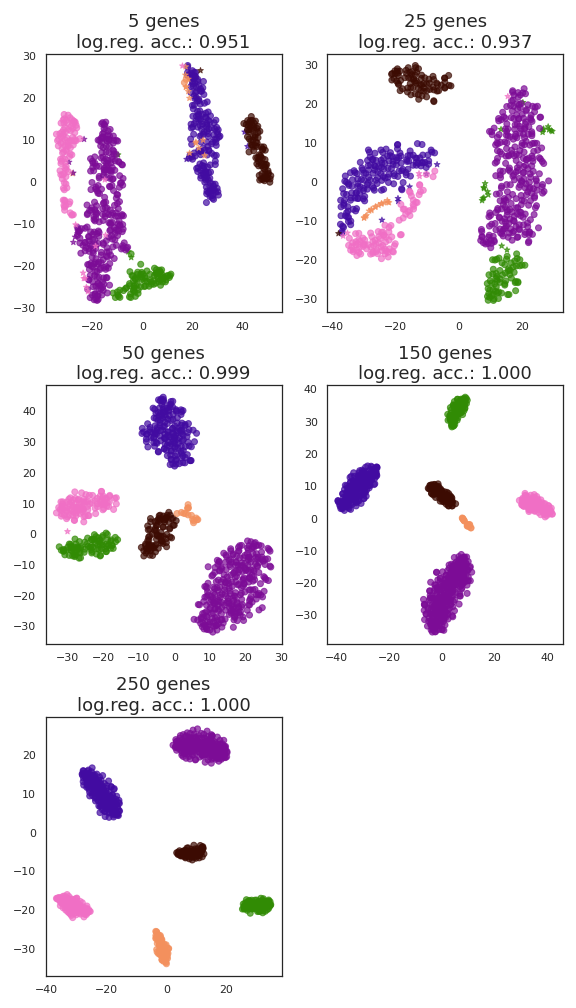
\includegraphics[width=\linewidth]{figs/TSNE_complex.png}
  \caption{\small t-SNE performance on the complex Splatter data-sets}
  \label{fig:tsne_complex}
\end{subfigure}\hspace{30px}%
\begin{subfigure}{.3\textwidth}
  \centering
  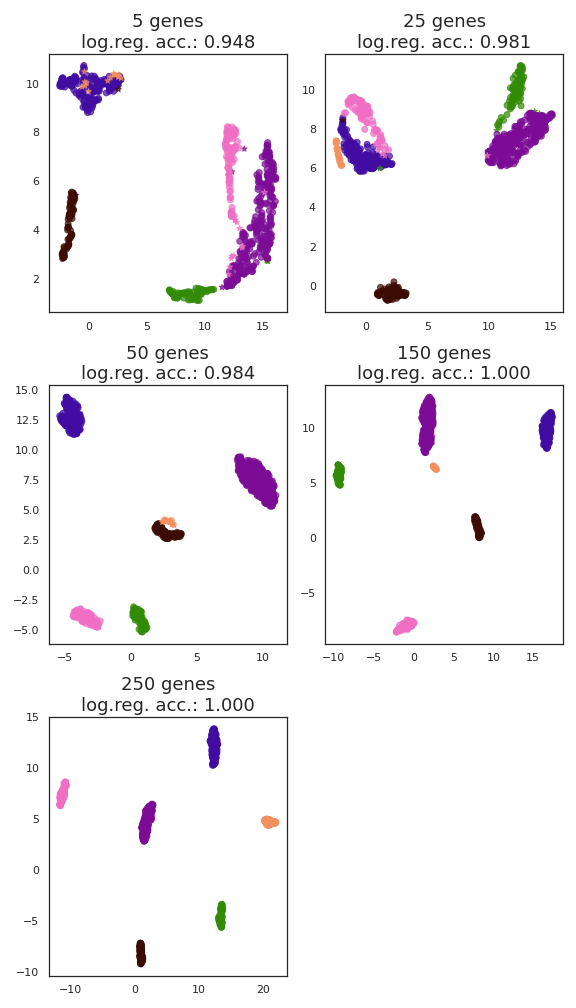
\includegraphics[width=\linewidth]{figs/UMAP_complex.png}
  \caption{\small UMAP performance on the complex Splatter data-sets}
  \label{fig:umap_complex}
\end{subfigure}
\small
\caption[t-SNE and UMAP performance on the Splatter data-sets.]{\small \textbf{t-SNE and UMAP performance on the Splatter data-sets.} \small The resulting plots when analyzing the simple Splatter data-sets with t-SNE (a) and UMAP (b) and when analyzing the complex Splatter data-sets with t-SNE (c) and UMAP (d). Colours indicate different cell types. Data-points that were predicted correctly by the logistic regression are plotted with dots, incorrect predictions are plotted with stars.}
\label{fig:baseline_splatter}
\end{figure}



\begin{figure}
    \centering
    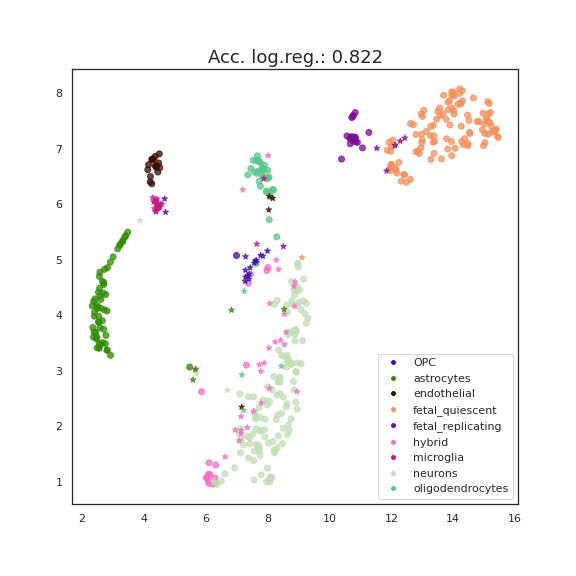
\includegraphics[width=.6\linewidth]{figs/darmanis_UMAP_logres.png}
    \caption[UMAP results of the Darmanis data-set.]{\small \textbf{UMAP results of the Darmanis data-set.} \small An accuracy of $0.822$ was measured after performing a logistic regression with a 5-fold cross validation. Colours indicate different cell types. Data-points that were predicted correctly by the logistic regression are plotted with dots, incorrect predictions are plotted with stars.}
    \label{fig:darmanis_umap}
\end{figure}

\begin{figure}
    \centering
    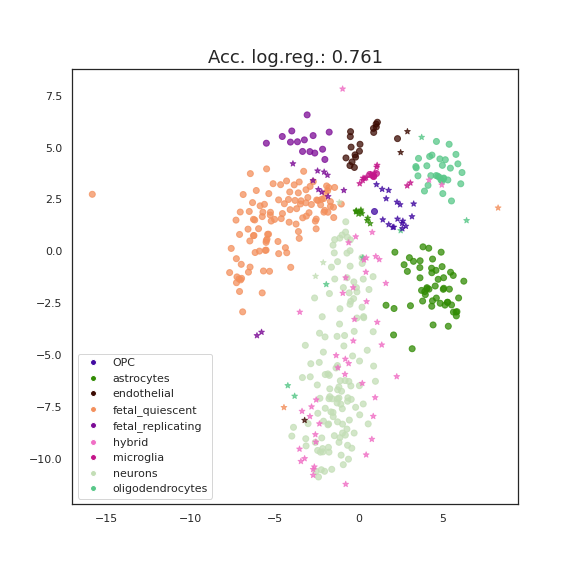
\includegraphics[width=.6\linewidth]{figs/darmanis_tsne_logres.png}
    \caption[t-SNE results of the Darmanis data-set.]{\small \textbf{t-SNE results of the Darmanis data-set.} \small An accuracy of $0.761$ was measured after performing a logistic regression with a 5-fold cross validation. Colours indicate different cell types. Data-points that were predicted correctly by the logistic regression are plotted with dots, incorrect predictions are plotted with stars.}
    \label{fig:darmanis_tsne}
\end{figure}



\begin{figure}
    \centering
    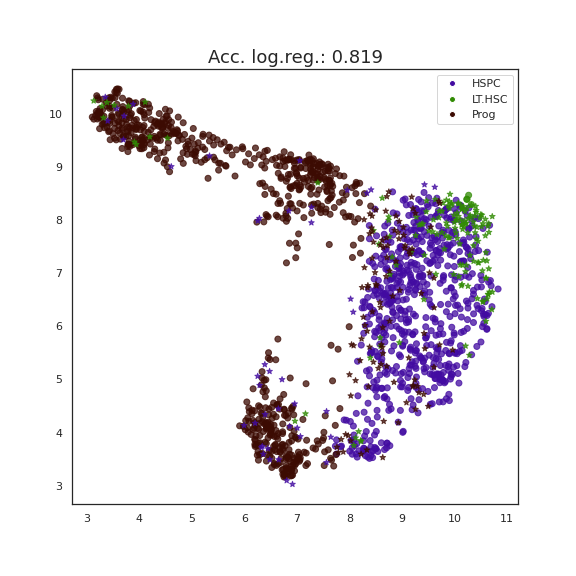
\includegraphics[width=.6\linewidth]{figs/nestorowa_UMAP_logres.png}
    \caption[UMAP results of the Nestorowa data-set.]{\small \textbf{UMAP results of the Nestorowa data-set.} \small An accuracy of $0.819$ was measured after performing a logistic regression with a 5-fold cross validation. Colours indicate different cell types. Data-points that were predicted correctly by the logistic regression are plotted with dots, incorrect predictions are plotted with stars.}
    \label{fig:nestorowa_umap}
\end{figure}

\begin{figure}
    \centering
    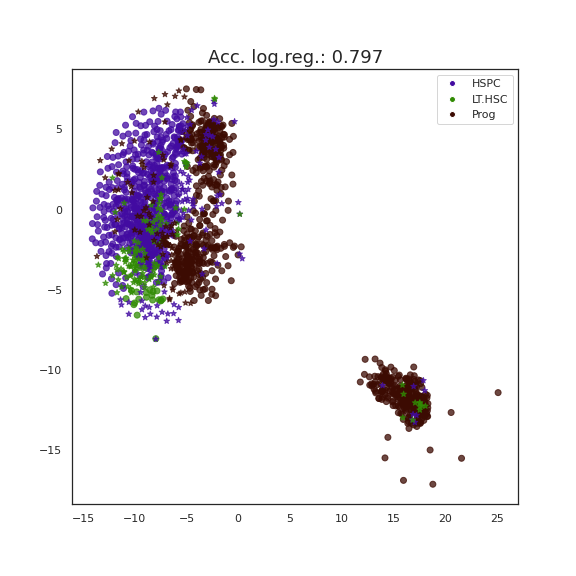
\includegraphics[width=.6\linewidth]{figs/nestorowa_tsne_logres.png}
    \caption[t-SNE results of the Nestorowa data-set.]{\small \textbf{t-SNE results of the Nestorowa data-set.} \small An accuracy of $0.797$ was measured after performing a logistic regression with a 5-fold cross validation. Colours indicate different cell types. Data-points that were predicted correctly by the logistic regression are plotted with dots, incorrect predictions are plotted with stars.}
    \label{fig:nestorowa_tsne}
\end{figure}
